\hypertarget{introduccion}{%
\section{Introducción}\label{introduccion}}

Escribir programas (o programar) es una actividad muy creativa y
gratificante. Puedes escribir programas por muchas razones, que pueden
ir desde mantenerte activo resolviendo un problema de análisis de datos
complejo hasta hacerlo por pura diversión ayudando a otros a resolver un
enigma. Este libro asume que \emph{todo el mundo} necesita saber
programar, y que una vez que aprendas a programar ya encontrarás qué
quieres hacer con esas habilidades recién adquiridas.

En nuestra vida diaria estamos rodeados de ordenadores, desde equipos
portátiles (laptops) hasta teléfonos móviles. Podemos pensar en esos
ordenadores como nuestros ``asistentes personales'', que pueden ocuparse
de muchas tareas por nosotros. El hardware en los equipos que usamos
cada día está diseñado esencialmente para hacernos la misma pregunta de
forma constante, ``¿Qué quieres que haga ahora?''.

Los programadores suelen añadir un sistema operativo y un conjunto de
aplicaciones al hardware y así nos proporcionan un Asistente Digital
Personal que es bastante útil y capaz de ayudarnos a realizar una gran
variedad de tareas.

Nuestros equipos son rápidos y tienen grandes cantidades de memoria.
Podrían resultar-no muy útiles si tan solo supiéramos qué idioma
utilizar para explicarle al ordenador qué es lo que queremos que ``haga
ahora''. Si conociéramos ese idioma, podríamos pedirle al aparato que
realizase en nuestro lugar, por ejemplo, tareas repetitivas.
Precisamente el tipo de cosas que los ordenadores saben hacer mejor
suelen ser el tipo de cosas que las personas encontramos pesadas y
aburridas.

Por ejemplo, mira los primeros tres párrafos de este capítulos y dime
cuál es la palabra que más se repite, y cuántas veces se ha utilizado.
Aunque seas capaz de leer y comprender las palabras en pocos segundos,
contarlas te resultará casi doloroso, porque la mente humana no fue
diseñada para resolver ese tipo de problemas. Para un ordenador es justo
al revés, leer y comprender texto de un trozo de papel le sería difícil,
pero contar las palabras y decirte cuántas veces se ha repetido la más
utilizada le resulta muy sencillo.

Nuestro ``asistente de análisis de información personal'' nos dirá
enseguida que la palabra ``que'' se usó ocho veces en los primeros tres
párrafos de este capítulo.

\begin{Verbatim}[frame=single]
>>> python words.py
  Escribe el nombre del fichero de texto: primeros-3-parrafos.txt
  Es la palabra: 'que'
  Aparece 8 veces
\end{Verbatim}


El hecho de que los ordenadores sean buenos en aquellas cosas en las que
los humanos no lo son es el motivo por el que necesitas aprender a
hablar el ``idioma de los ordenadores''. Una vez que aprendas este nuevo
lenguaje, podrás delegar tareas mundanas a tu compañero (el ordenador),
lo que te dejará más tiempo para ocuparte de las cosas para las que sólo
tú estás capacitado. Tú pondrás la creatividad, intuición y el ingenio
en esa alianza.

Para ejecutar una tarea o resolver un problema utilizamos algoritmos. 

\begin{definition}
Un \textbf{algoritmo} es una secuencia de instrucciones especificas de las acciones
que ha de ejecutar y en qué orden para completar una tarea determinada.
\end{definition}

Por ejemplo, una receta para hacer paella es como un algoritmo que
consiste de una secuencia de pasos que tienes que tomar para hacer una
paella valenciana.
%
Otros algoritmos que conocemos son por ejemplo los pasos que nos enseñan
en el colegio para multiplicar (mira la Figure \ref{fig:multiplicar}). 

\begin{figure}
    \centering
    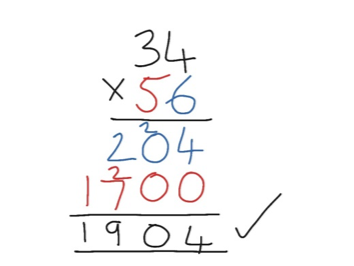
\includegraphics[width=0.5\textwidth]{images/multiplicar.pdf}
    \caption{Algoritmo para multiplicar 34 con 56}
    \label{fig:multiplicar}
\end{figure}


\begin{itemize}[nosep]
\item
  paso 1: ponemos el multiplicando (34) arriba y el multiplicador (56)
  abajo
\item
  paso 2: multiplicar las unidades del multiplicador por el
  multiplicando y el resultado escribirlo en la fila de abajo.
\item
  paso 3: multiplicar las decenas del multiplicador por el multiplicando
  y el resultado escribirlo en la fila de abajo pero desplazado una
  posición a la izquierda.
\item
  paso 4: sumar los dos productos
\end{itemize}

\hypertarget{arquitectura-hardware-de-los-ordenadores}{%
\section{Arquitectura hardware de los
ordenadores}\label{arquitectura-hardware-de-los-ordenadores}}

\index{hardware} \index{hardware!arquitectura}

Antes de que empecemos a aprender el lenguaje que deberemos hablar para
darle instrucciones a los ordenadores para desarrollar software,
tendremos que aprender un poco acerca de cómo están construidos esas
máquinas. Si desmontaras tu ordenador o \emph{smartphone} y mirases
dentro con atención, encontrarías diferentes componentes
como en la Figura \ref{fig:arch}.

\begin{figure}
    \centering
    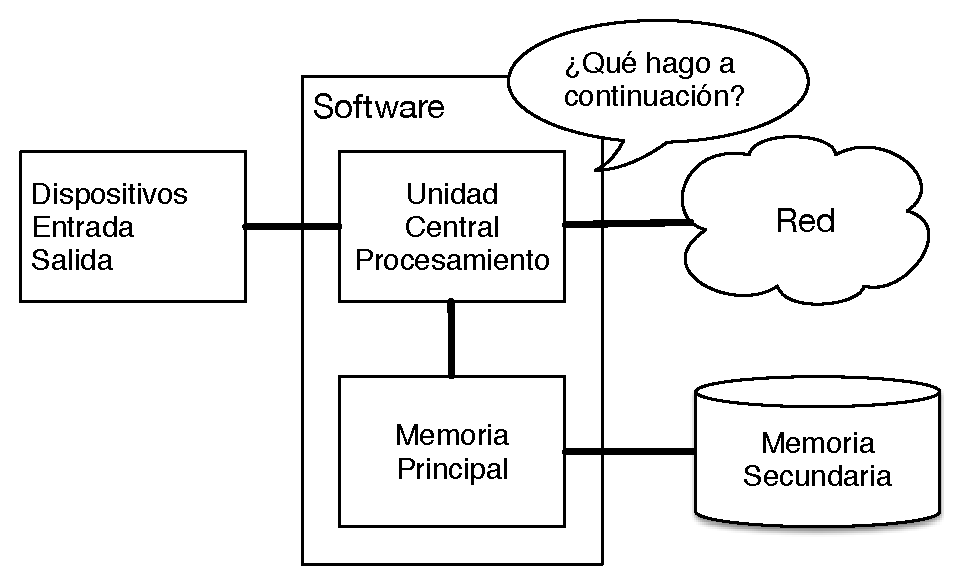
\includegraphics[width=0.5\textwidth]{images/arch.eps}
    \caption{La arquitectura de un ordenador}
    \label{fig:arch}
\end{figure}


Las definiciones de alto nivel de esos componentes son las siguientes:

\begin{itemize}[nosep]
\item
  La \emph{Unidad Central de Procesamiento} (o
  CPU\footnote{Central Processing Unit en inglés
  (N. del T.).}) es el componente del ordenador diseñado para estar
  obsesionado con el ``¿qué hago a continuación?'' (o ``what's next?''
  en ingles). Si tu equipo está dentro de la clasificación de 3.0
  Gigahercios, significa que la CPU preguntará ``¿qué hago a
  continuación?'' tres mil millones de veces por segundo. Vas a tener
  que aprender a hablar muy rápido para mantener el ritmo de la CPU.
\item
  La \emph{Memoria Principal} se usa para almacenar la información que
  la CPU necesita de forma inmediata. La memoria principal es casi tan
  rápida como la CPU. Pero la información almacenada en la memoria
  principal desaparece cuando se apaga el equipo.
\item
  La \emph{Memoria Secundaria} también se utiliza para almacenar
  información, pero es mucho más lenta que la memoria principal. La
  ventaja de la memoria secundaria es que puede almacenar la información
  incluso cuando el equipo está apagado. Algunos ejemplos de memoria
  secundaria serían las unidades de disco o las memorias flash (que
  suelen encontrarse en los \emph{pendrives} USB y en los reproductores
  de música portátiles).
\item
  Los \emph{Dispositivos de Entrada y Salida} son simplemente la
  pantalla, teclado, ratón, micrófono, altavoz, \emph{touchpad}, etc.
  Incluyen cualquier modo de interactuar con un ordenador.
\item
  Actualmente, casi todos los equipos tienen una \emph{Conexión de Red}
  para recibir información dentro de una red. Podemos pensar en una red
  como en un lugar donde almacenar y recuperar datos de forma muy lenta,
  que puede no estar siempre ``activo''. Así que, en cierto sentido, la
  red no es más que un tipo de \emph{Memoria Secundaria} más lenta y a
  veces poco fiable.
\end{itemize}

Aunque la mayoría de los detalles acerca de cómo funcionan estos
componentes es mejor dejársela a los constructores de equipos, resulta
útil disponer de cierta terminología para poder referirnos a ellos a la
hora de escribir nuestros programas.

Como programador, tu trabajo es usar y orquestar cada uno de esos
recursos para resolver el problema del que tengas que ocuparte y
analizar los datos de los que dispongas para encontrar la solución. Como
programador estarás casi siempre ``hablando'' con la CPU y diciéndole
qué es lo siguiente que debe hacer. A veces le tendrás que pedir a la
CPU que use la memoria principal, la secundaria, la red, o los
dispositivos de entrada/salida.

\begin{figure}
\centering
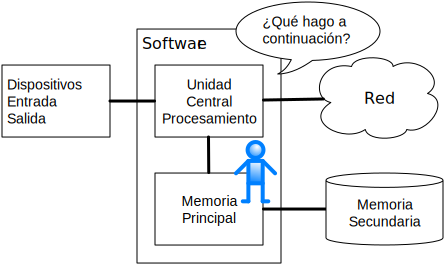
\includegraphics[width=0.5\textwidth]{images/arch2}
\caption{¿Dónde estás tu como programador?}
\label{fig:donde-estas}
\end{figure}

Tú deberás ser la persona que responda a la pregunta ``¿Qué hago
ahora?'' de la CPU. Pero sería muy incómodo encogerse uno mismo hasta
los 5 mm. de altura e introducirse dentro del ordenador sólo para poder
dar una orden tres mil millones de veces por segundo. Así que en vez de
eso, tendrás que escribir las instrucciones por adelantado. Esas
instrucciones almacenadas reciben el nombre de \emph{programa} y el acto
de escribirlas y encontrar cuáles son las instrucciones adecuadas,
\emph{programar}.

\hypertarget{programacion}{%
\section{Programación}\label{programacion}}

Crear programas útiles, elegantes e inteligentes para que los usen
otros, es una actividad muy creativa. La Programación es la disciplina
relacionada con:

\begin{itemize}[nosep]
\item
  La resolución de problemas mediante algoritmos
\item
  Codificar el algoritmo como programa en un determinado lenguaje
\item
  Testear (o probar) el programa ejecutándolo con el ordenador
\end{itemize}

En esta asignatura intentaremos convertirte en una persona
experta en el arte de programar. Al terminar, te habrás convertido en un
\emph{programador} - tal vez no uno profesional, pero al menos tendrás
la capacidad de encarar un problema de análisis de datos/información y
desarrollar algoritmos/programas para resolverlo.

\index{resolución de un problema}

En cierto modo, necesitas las siguientes capacidades para ser
programador:

\begin{itemize}[nosep]
\item
  Primero, necesitas saber un lenguaje de programación (Python) - debes
  conocer su vocabulario y su gramática. Debes ser capaz de deletrear
  correctamente las palabras en ese nuevo lenguaje y saber construir
  ``frases'' bien formadas.
\item
  Segundo, debes ``contar una historia''. Al escribir un \emph{relato}
  en languaje natural, combinas palabras y frases para comunicar una
  \emph{idea} al lector. Hay una cierta técnica y arte en la
  construcción de un relato, y la habilidad para escribir relatos mejora
  escribiendo y recibiendo cierta respuesta. En programación, nuestro
  \emph{algoritmo} es el ``relato'' que quieres escribir y el
  \emph{problema} que estás tratando de resolver es la ``idea''.
\item
  Tercero, necesitas verificar que el lector interprete bien tu historia
  para que no haya mal entendidos. En programación eso significa que
  tenemos que ejecutar {\em tests} con nuestro programa, ejecutándolo para
  asegurar que haga lo que queremos que haga.
\end{itemize}

Una vez que aprendas un lenguaje de programación como Python,
encontrarás mucho más fácil aprender un segundo lenguaje como JavaScript
o C++. Cada nuevo lenguaje tiene un vocabulario y gramática muy
diferentes, pero la técnica de resolución de problemas será la misma en
todos ellos.

Aprenderás el ``vocabulario'' y ``frases'' de Python bastante rápido. Lo que te
llevará más tiempo es ser capaz de escribir un programa coherente para
resolver un problema totalmente nuevo porque para eso se necesita practicar 
el \textbf{pensamiento computacional}, o ''\textbf{computational thinking}'' en inglés.
\index{pensamiento computacional}\index{computational thinking}

El pensamiento computacional se refiere a un enfoque mental y analítico para resolver problemas que involucra habilidades fundamentales tomadas de la ciencia de la computación. Estas habilidades pueden ser aplicadas en una variedad de contextos y no están limitadas exclusivamente a la programación o la tecnología. El pensamiento computacional implica abordar problemas de manera:

\begin{itemize}
\item estructurada y lógica, 
\item formulando soluciones de manera eficiente y efectiva,
\item identificando patrones y relaciones, 
\item descomponiendo problemas complejos en componentes más pequeños y manejables,
\item evaluando la solucion
\end{itemize}

Los componentes clave del pensamiento computacional incluyen:

\begin{description}
\item[Algoritmos]: Desarrollar pasos secuenciales y lógicos para resolver un problema, siguiendo una serie de instrucciones claras y definidas.

\item[Reconocimiento de patrones]: Identificar similitudes y tendencias en los datos o situaciones para poder generalizar y aplicar soluciones a problemas similares.

\item[Descomposición]: Dividir un problema en partes más pequeñas y manejables para entenderlo mejor y abordarlo de manera más efectiva.


\item[Abstracción]: Centrarse en los detalles más relevantes y eliminar la información innecesaria para simplificar la comprensión y la solución del problema.
\end{description}

El pensamiento computacional no se limita a la programación, aunque la programación es una manifestación tangible de este enfoque. Puede ser aplicado en una amplia gama de campos, como la resolución de problemas matemáticos, la toma de decisiones empresariales, la optimización de procesos, la ciencia de datos, la resolución de problemas científicos, la creatividad en el diseño, y mucho más. Fomentar el pensamiento computacional puede ayudar a las personas a enfrentar desafíos complejos de manera más estructurada y efectiva, independientemente de su campo de interés.

Pero por ahora, vamos a empezar con enseñar programación de forma
muy similar a como se enseña a escribir. Se empieza leyendo y explicando
programas, luego se escriben programas sencillos, y a continuación se
van escribiendo programas progresivamente más complejos con el tiempo.
En algún momento ``encuentras tu musa'', empiezas a descubrir los
patrones por ti mismo y empiezas a ver casi de forma instintiva cómo
abordar un problema y escribir un programa para resolverlo. Y una vez
alcanzado ese punto, la programación se convierte en un proceso muy
placentero y creativo.

Comenzaremos con el vocabulario y la estructura de los programas en
Python. 

\hypertarget{palabras-y-frases}{%
\section{Palabras y frases}\label{palabras-y-frases}}

\index{lenguaje de programación} \index{lenguaje!programación}

A diferencia de los lenguajes humanos, el vocabulario de Python es en
realidad bastante reducido. Llamamos a este ``vocabulario'' las
``palabras reservadas''. Se trata de palabras que tienen un significado
muy especial para Python. Cuando Python se encuentra estas palabras en
un programa, sabe que sólo tienen un único significado para él. Más
adelante, cuando escribas programas, podrás usar tus propias palabras
con significado, que reciben el nombre de \emph{variables}. Tendrás gran
libertad a la hora de elegir los nombres para tus variables, pero no
podrás utilizar ninguna de las palabras reservadas de Python como nombre
de una variable.

Cuando se entrena a un perro, se utilizan palabras especiales como
``siéntate'', ``quieto'' y ``tráelo''. Cuando te diriges a un perro y no
usas ninguna de las palabras reservadas, lo único que consigues es que
se te quede mirando con cara extrañada, hasta que le dices una de las
palabras que reconoce. Por ejemplo, si dices, ``Me gustaría que más
gente saliera a caminar para mejorar su salud general'', lo que la
mayoría de los perros oirían es: ``bla bla bla \emph{caminar} bla bla
bla bla.''. Eso se debe a que ``caminar'' es una palabra reservada en el
lenguaje del perro. Seguramente habrá quien apunte que el lenguaje entre
humanos y gatos no dispone de palabras reservadas\footnote{\url{http://xkcd.com/231/}}.

Las palabras reservadas en el lenguaje que utilizan los humanos para
hablar con Python son, entre otras, las siguientes:

\begin{verbatim}
and       del       global      not       with
as        elif      if          or        yield
assert    else      import      pass      
break     except    in          raise
class     finally   is          return
continue  for       lambda      try
def       from      nonlocal    while    
\end{verbatim}

Es decir, a diferencia de un perro, Python ya está completamente
entrenado. Cada vez le digas ``inténtalo'', Python lo intentará una vez
tras otra sin desfallecer\footnote{
En inglés "inténtalo" es "try", que es también una palabra reservada dentro del
lenguaje Python (N. del T.).}.

Aprenderemos cuáles son las palabras reservadas y cómo utilizarlas en su
momento, pero por ahora nos centraremos en el equivalente en Python de
``habla'' (en el lenguaje humano-perro). Lo bueno de pedirle a Python
que hable es que podemos incluso indicarle lo que debe decir, pasándole
un mensaje entre comillas:

\begin{Verbatim}[frame=single]
    print('¡Hola, mundo!')
\end{Verbatim}

Y ya acabamos de escribir nuestra primera oración sintácticamente
correcta en Python. La frase comienza con la función \emph{print}
seguida de la cadena de texto que hayamos elegido dentro de comillas
simples. Las comillas simples y dobles cumplen la misma función; la
mayoría de las personas usan las comillas simples, excepto cuando la
cadena de texto contiene también una comilla simple (que puede ser un
apóstrofo).

\section{Instalando Thonny, un entorno integrado de desarrollo (IDE)}

Antes de que puedas conversar con Python, deberás instalar el software necesario en tu ordenador y aprender a iniciar Python en ella. En este asignatura usamos {\em Thonny} (\url{https://thonny.org/}) un entorno integrado de desarrollo (IDE) pensado para principiantes. Es sencillo de usar, consume pocos recursos y además ya incorpora el interprete de Python versión 3.


La pantalla de Thonny está compuesta de varias ventanas. Esta presentación es configurable pero nosotros usaremos la mayoría de veces la disposición que se ve en la Figura~\ref{fig:Thonny} y que explicamos a continuación.

\begin{figure}
	\centering
	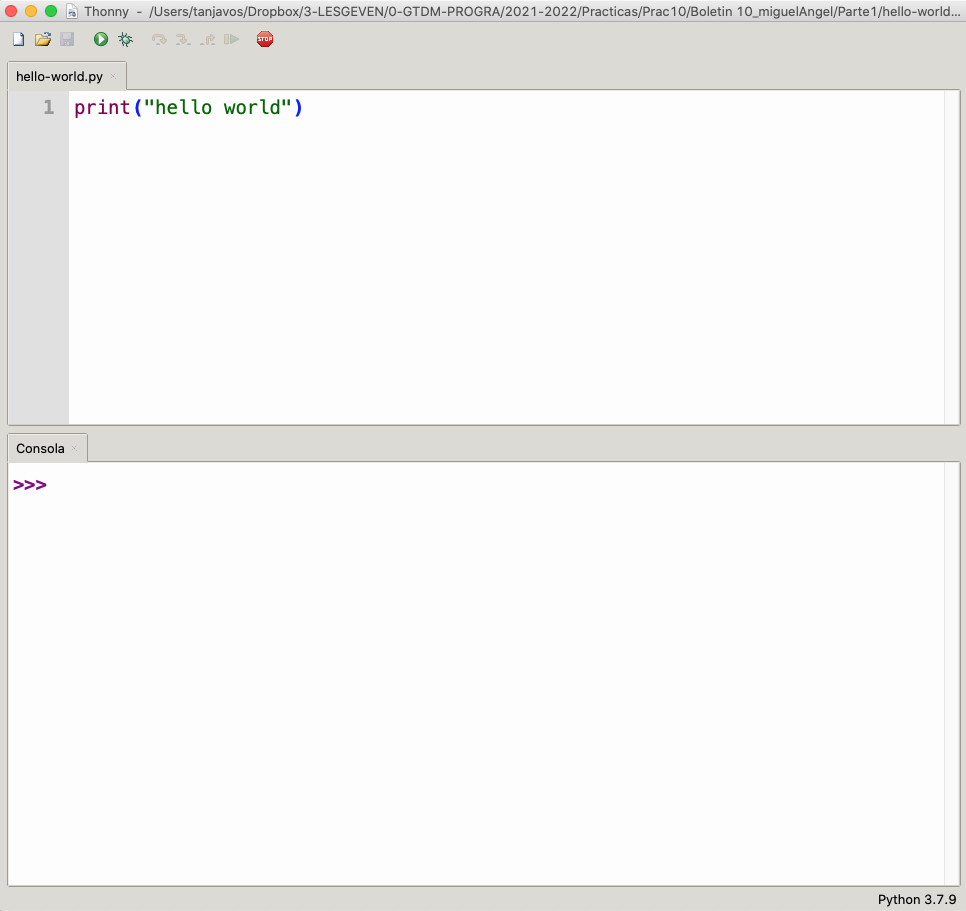
\includegraphics[width=.85\textwidth]{images/Thonny.png}
	\caption{Interfaz de Thonny}
	\label{fig:Thonny}
\end{figure}

En la parte superior encontramos diferentes botones para por ejemplo abrir, ejecutar y parar programas.

Debajo de ella nos encontramos las ventanas principales de trabajo: 

\begin{itemize}[nosep]
 \item  el editor de código donde podremos crear y editar nuestros programas. 
 \item debajo de ella se encuentra el shell o consola de ejecución, mediante ella nos podremos conversar con Python y nuestros programas, ya sea introduciendo datos o viendo los resultados que este presenta. También servirá para ejecutar de forma interactiva ordenes de Python.
 
 El indicador \verb|>>>| es el modo que tiene el intérprete de Python de preguntarte, ''¿Qué quieres que haga ahora?''. Python está ya preparado para mantener una
conversación contigo. Todo lo que tienes que saber es cómo hablar en su idioma.
\end{itemize}


\hypertarget{conversando-con-python}{%
\section{Conversando con Python}\label{conversando-con-python}}


Supongamos por ejemplo que aún no conoces ni las palabras ni frases más sencillas
de Python. Puede que quieras utilizar el método clásico de los
astronautas cuando aterrizan en un planeta lejano e intentan hablar con los
habitantes de ese mundo:

\begin{Verbatim}[frame=single]
>>> Vengo en son de paz, por favor llévame ante tu líder
      File "<stdin>", line 1
        Vengo en son de paz, por favor llévame ante tu líder
              ^
    SyntaxError: invalid syntax
>>>
\end{Verbatim}


Esto no se ve bien. A menos que pienses en algo rápidamente, los habitantes del planeta sacarán sus lanzas, te ensartarán, te asarán sobre el fuego y al final les servirás de cena.

Por suerte has leído las secciones anteriores durante tus viajes, así que lo abres precisamente por esta página y pruebas de nuevo:

\begin{Verbatim}[frame=single]
>>> print('¡Hola, mundo!')
    ¡Hola, mundo!
\end{Verbatim}

Esto tiene mejor aspecto, de modo que intentas comunicarte un poco más:

\begin{Verbatim}[frame=single]
>>> print('Usted debe ser el dios legendario que viene del cielo')
    Usted debe ser el dios legendario que viene del cielo
>>> print('Hemos estado esperándole durante mucho tiempo')
    Hemos estado esperándole durante mucho tiempo
>>> print('La leyenda dice que debe estar usted muy rico con mostaza')
    La leyenda dice que debe estar usted muy rico con mostaza
>>> print 'Tendremos un festín esta noche a menos que diga
    File "<stdin>", line 1
        print 'Tendremos un festín esta noche a menos que diga
                                                             ^
    SyntaxError: Missing parentheses in call to 'print'
    >>>
\end{Verbatim}

La conversación fue bien durante un rato, pero en cuanto cometiste el
más mínimo fallo al utilizar el lenguaje Python, Python volvió a sacar
las lanzas.

En este momento, te habrás dado cuenta que a pesar de que Python es
tremendamente complejo y poderoso, y muy estricto en cuanto a la
sintaxis que debes usar para comunicarte con él, Python \emph{no} es
inteligente. En realidad estás solamente manteniendo una conversación
contigo mismo; eso sí, usando una sintaxis adecuada.

En cierto modo, cuando utilizas un programa escrito por otra persona, la
conversación se mantiene entre tú y el programador, con Python actuando
meramente de intermediario. Python es una herramienta que permite a los
creadores de programas expresar el modo en que la conversación
supuestamente debe fluir. Y dentro de unos pocos capítulos más, serás
uno de esos programadores que utilizan Python para hablar con los
usuarios de tu programa.

Antes de que abandonemos nuestra primera conversación con el intérprete
de Python, deberías aprender cual es el modo correcto de decir ``adiós''
al interactuar con los habitantes del Planeta Python:

\begin{Verbatim}[frame=single]
>>> adiós
    Traceback (most recent call last):
      File "<stdin>", line 1, in <module>
    NameError: name 'adiós' is not defined
>>> if you don't mind, I need to leave
      File "<stdin>", line 1
        if you don't mind, I need to leave
                 ^
    SyntaxError: invalid syntax
>>> quit()
\end{Verbatim}

Te habrás fijado en que el error es diferente en cada uno de los dos
primeros intentos. El segundo error es diferente porque \emph{if} es una
palabra reservada, y cuando Python la ve, cree que estamos intentando
decirle algo, pero encuentra la sintaxis de la frase incorrecta.

La forma correcta de decirle ``adiós'' a Python es introducir
\emph{quit()} en el símbolo indicador del sistema
\texttt{\textgreater{}\textgreater{}\textgreater{}}. Seguramente te
hubiera llevado un buen rato adivinarlo, así que tener este libro a mano
probablemente te haya resultado útil.

\hypertarget{terminologuxeda-intuxe9rprete-y-compilador}{%
\section{Terminología: intérprete y
compilador}\label{terminologuxeda-intuxe9rprete-y-compilador}}

Python es un lenguaje \emph{de alto nivel}, pensado para ser
relativamente sencillo de leer y escribir para las personas, y fácil de
leer y procesar para las máquinas. Otros lenguajes de alto nivel son
Java, C++, PHP, Ruby, Basic, Perl, JavaScript, y muchos más. El hardware
real que está dentro de la Unidad Central de Procesamiento (CPU), no
entiende ninguno de esos lenguajes de alto nivel.

La CPU entiende únicamente un lenguaje llamado \emph{lenguaje de
máquina} o \emph{código máquina}. El código máquina es muy simple y
francamente muy pesado de escribir, ya que está representado en su
totalidad por solamente ceros y unos:

\begin{verbatim}
    001010001110100100101010000001111
    11100110000011101010010101101101
    ...
\end{verbatim}

El código máquina parece bastante sencillo a simple vista, dado que sólo
contiene ceros y unos, pero su sintaxis es incluso más compleja y mucho
más enrevesada que la de Python, razón por la cual muy pocos
programadores escriben en código máquina. En vez de eso, se han creado
varios programas traductores para permitir a los programadores escribir
en lenguajes de alto nivel como Python o Javascript, y son esos
traductores quienes convierten los programas a código máquina, que es lo
que ejecuta en realidad la CPU.

Dado que el código máquina está ligado al hardware de la máquina que lo
ejecuta, ese código no es \emph{portable} (trasladable) entre equipos de
diferente tipo. Los programas escritos en lenguajes de alto nivel pueden
ser trasladados entre distintas máquinas usando un intérprete diferente
en cada una de ellas, o recompilando el código para crear una versión
diferente del código máquina del programa para cada uno de los tipos de
equipo.

Esos traductores de lenguajes de programación forman dos categorías
generales: (1) intérpretes y (2) compiladores.

Un \emph{intérprete} lee el código fuente de los programas tal y como ha
sido escrito por el programador, lo analiza, e interpreta sus
instrucciones sobre la marcha. Python es un intérprete y cuando lo
estamos ejecutando de forma interactiva, podemos escribir una línea de
Python (una frase), y este la procesa de forma inmediata, quedando listo
para que podamos escribir otra línea.

Algunas de esas líneas le indican a Python que tú quieres que recuerde
cierto valor para utilizarlo más tarde. Tenemos que escoger un nombre
para que ese valor sea recordado y usaremos ese nombre simbólico para
recuperar el valor más tarde. Utilizamos el término \emph{variable} para
denominar las etiquetas que usamos para referirnos a esos datos
almacenados.

\begin{Verbatim}[frame=single]
>>> x = 6
>>> print(x)
  6
>>> y = x * 7
>>> print(y)
  42
>>>
\end{Verbatim}
En este ejemplo, le pedimos a Python que recuerde el valor seis y use la
etiqueta \emph{x} para que podamos recuperar el valor más tarde.
Comprobamos que Python ha guardado de verdad el valor usando
\emph{print}. Luego le pedimos a Python que recupere \emph{x}, lo
multiplique por siete y guarde el valor calculado en \emph{y}.
Finalmente, le pedimos a Python que escriba el valor actual de \emph{y}.

A pesar de que estamos escribiendo estos comandos en Python línea a
línea, Python los está tratando como una secuencia ordenada de
sentencias, en la cual las últimas frases son capaces de obtener datos
creados en las anteriores. Estamos, por tanto, escribiendo nuestro
primer párrafo sencillo con cuatro frases en un orden lógico y útil.

La esencia de un \emph{intérprete} consiste en ser capaz de mantener una
conversación interactiva como la mostrada más arriba. Un
\emph{compilador} necesita que le entreguen el programa completo en un
fichero, y luego ejecuta un proceso para traducir el código fuente de
alto nivel a código máquina, tras lo cual coloca ese código máquina
resultante dentro de otro fichero para su ejecución posterior.

En sistemas Windows, a menudo esos ejecutables en código máquina tienen
un sufijo o extensión como ``.exe'' o ``.dll'', que significan
``ejecutable'' y ``librería de enlace dinámico'' (\emph{dynamic link
library}) respectivamente. En Linux y Macintosh, no existe un sufijo que
identifique de manera exclusiva a un fichero como ejecutable.

Si abrieras un fichero ejecutable con un editor de texto, verías algo
complemente disparatado e ilegible:

\begin{verbatim}
    ^?ELF^A^A^A^@^@^@^@^@^@^@^@^@^B^@^C^@^A^@^@^@\xa0\x82
    ^D^H4^@^@^@\x90^]^@^@^@^@^@^@4^@ ^@^G^@(^@$^@!^@^F^@
    ^@^@4^@^@^@4\x80^D^H4\x80^D^H\xe0^@^@^@\xe0^@^@^@^E
    ^@^@^@^D^@^@^@^C^@^@^@^T^A^@^@^T\x81^D^H^T\x81^D^H^S
    ^@^@^@^S^@^@^@^D^@^@^@^A^@^@^@^A\^D^HQVhT\x83^D^H\xe8
    ....
\end{verbatim}

No resulta fácil leer o escribir código máquina, pero afortunadamente
disponemos de \emph{intérpretes} y \emph{compiladores} que nos permiten
escribir en lenguajes de alto nivel, como Python o C.

Llegados a este punto en la explicación acerca de los compiladores e
intérpretes, seguramente te estarás preguntando algunas cosas acerca del
propio intérprete de Python. ¿En qué lenguaje está escrito? ¿Está
escrito en un lenguaje compilado? Cuando escribimos ``python'', ¿qué
ocurre exactamente?

El intérprete de Python está escrito en un lenguaje de alto nivel
llamado ``C''. En realidad, puedes ver el código fuente del intérprete
de Python acudiendo a \href{http://www.python.org}{www.python.org} e
incluso modificarlo a tu gusto. Quedamos, pues, en que Python es en sí
mismo un programa y que está compilado en código máquina. Cuando
instalaste Python en tu ordenador (o el vendedor lo instaló), colocaste
una copia del código máquina del programa Python traducido para tu
sistema. En Windows, el código máquina ejecutable para el intérprete de
Python es probablemente un fichero con un nombre como:

\begin{verbatim}
    C:\Python35\python.exe
\end{verbatim}

En realidad, eso ya es más de lo que necesitas saber para ser un
programador en Python, pero algunas veces vale la pena contestar estas
pequeñas dudas recurrentes justo al principio.

\hypertarget{escribiendo-un-programa}{%
\section{Escribiendo un programa}\label{escribiendo-un-programa}}

Escribir comandos en el intérprete de Python es un buen modo de
experimentar con las capacidades de Python, pero no es lo más
recomendado a la hora de resolver problemas más complejos.

Cuando queremos escribir un programa, usamos un editor de texto para
escribir las instrucciones de Python en un fichero, que recibe el nombre
de \emph{script}. Por convención, los scripts de Python tienen nombres
que terminan en \texttt{.py}. En Thonny podemos usar el editor de código. 

\index{script}

Para ejecutar un programa en Thonny, podemos usar:

\begin{itemize}
    \item el botón de una flecha verde de la barra de herramientas
    \item el atajo de teclado F5
\end{itemize}
Es posible que Thonny pregunte la primera vez dónde guardar el programa si no lo hemos hecho antes. 

\begin{figure}
    \centering
    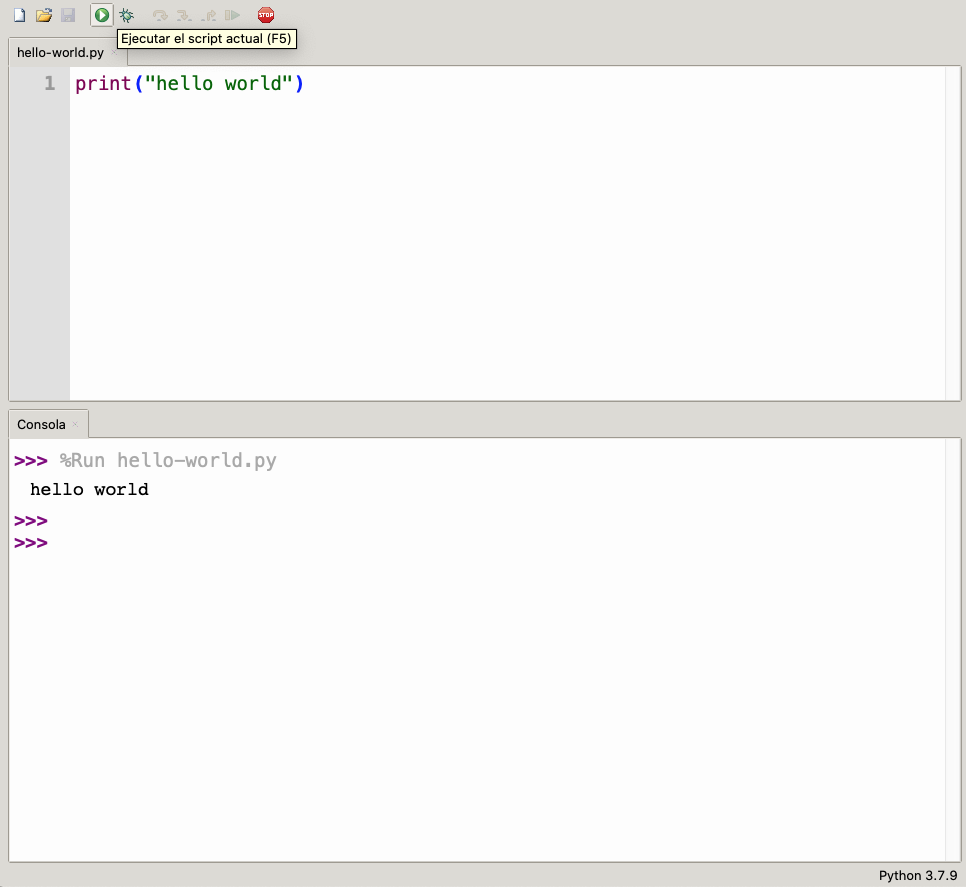
\includegraphics[width=.85\textwidth]{images/Thonny-execute.png}
    \caption{Para ejecutar: el botón de una flecha verde o F5 }
    \label{fig:thonny-execute}
\end{figure}


En la Figura~\ref{fig:thonny-execute} vemos que tradicionalmente, es el primer programa que escribes en un nuevo lenguaje
de programación se llama \verb|hello-world.py| porque todo lo que hace es mostrar las palabras \verb|hello world|(\verb|hola mundo|).  
Este es un ejemplo de una \textbf{instrucción print}, aunque
en realidad no imprime nada en papel.  Esta sentencia muestra un resultado en la
pantalla.  En este caso, el resultado es la frase \verb|hello world| como podemos ver en la Consola después de haber ejecutado el programa.
Las comillas en el programa marcan el principio y el final
del texto a visualizar: estas no aparecen en el resultado.
\index{comillas}
\index{sentencia!print}
\index{print, sentencia}




En la Figura \ref{fig:thonny-execute} vemos como hemos ejecutado el archivo \verb|hello-world.py| que contiene
un programa con una única línea de código que imprime en pantalla una cadena de texto.

Ejecutar un programa significa llamar al intérprete de Python y pedirle que lea el código fuente
desde el archivo \verb|hello-world.py|, en vez de esperar a que vayamos
introduciendo líneas de código Python de forma interactiva.

Habrás notado que cuando trabajamos con un fichero no necesitamos
incluir el comando \emph{quit()} al final del programa Python. Cuando
Python va leyendo tu código fuente desde un archivo, sabe que debe parar
cuando llega al final del fichero.

\hypertarget{quuxe9-es-un-programa}{%
\section{¿Qué es un programa?}\label{quuxe9-es-un-programa}}

\begin{definition}
Un \textbf{programa}, en su forma más básica, es una
secuencia de instrucciones o sentencias que han sido diseñadas para
hacer algo. 
\end{definition}

Nuestro sencillo script \verb|hello-world.py| es un programa.
Es un programa de una sola línea y no resulta particularmente útil, pero
si nos ajustamos estrictamente a la definición, se trata de un programa
en Python.

Tal vez resulte más fácil comprender qué es un programa pensando en un
problema que pudiera ser resuelto a través de un programa, y luego
estudiando cómo sería el programa que solucionaría ese problema.

Supongamos que estás haciendo una investigación de computación o
informática social en mensajes de Facebook, y te interesa conocer cual
es la palabra más utilizada en un conjunto de mensajes. Podrías imprimir
el flujo de mensajes de Facebook y revisar con atención el texto,
buscando la palabra más común, pero sería un proceso largo y muy
propenso a errores. Sería más inteligente escribir un programa en Python
para encargarse de la tarea con rapidez y precisión, y así poder emplear
el fin de semana en hacer otras cosas más divertidas.

Por ejemplo, fíjate en el siguiente texto, que trata de un payaso y un
coche. Estúdialo y trata de averiguar cual es la palabra más común y
cuántas veces se repite.

\begin{verbatim}
    el payaso corrió tras el coche y el coche se metió dentro de la tienda
    y la tienda cayó sobre el payaso y el coche
\end{verbatim}

Ahora imagina que haces lo mismo pero buscando a través de millones de
líneas de texto. Francamente, tardarías menos aprendiendo Python y
escribiendo un programa en ese lenguaje para contar las palabras que si
tuvieras que ir revisando todas ellas una a una.

Pero hay una noticia aún mejor, y es que ya hay un programa sencillo para encontrar cuál es la palabra más común dentro de un fichero de texto. 

\begin{python}
name = input('Escribe el nombre del fichero de texto: ')
handle = open(name, 'r')
counts = dict()

for line in handle:
    words = line.split()
    for word in words:
        counts[word] = counts.get(word, 0) + 1

bigcount = None
bigword = None
for word, count in list(counts.items()):
    if bigcount is None or count > bigcount:
        bigword = word
        bigcount = count

print("Es la palabra: " + bigword)
print("Aparece {} veces".format(bigcount))
\end{python}


No necesitas ni siquiera saber Python para usar este programa. Tendrás
que llegar hasta el tema de ficheros para entender por completo
las impresionantes técnicas de Python que se han utilizado para crearlo.
Ahora eres el usuario, puedes usar y testear el programa y
sorprenderte de sus habilidades y de cómo te permite ahorrar un montón de esfuerzo. Tan sólo tienes que escribir el código dentro del editor de código de Thonny y guárdalo en un fichero llamado \verb|words.py| y ejecutarlo ( o puedes descargar el código
fuente directamente desde PoliformaT). En Poliformat también encuentras 5 ficheros \verb|test1.txt| hasta \verb|test5.txt| que puedes usar para hacer testing del programa. En la Figura \ref{fig:Thonny-execute-words} puedes ver el resultado del primer test con el fichero \verb|test1.txt| que contiene el texto del payaso de más arriba.

\begin{figure}[t]
    \centering
    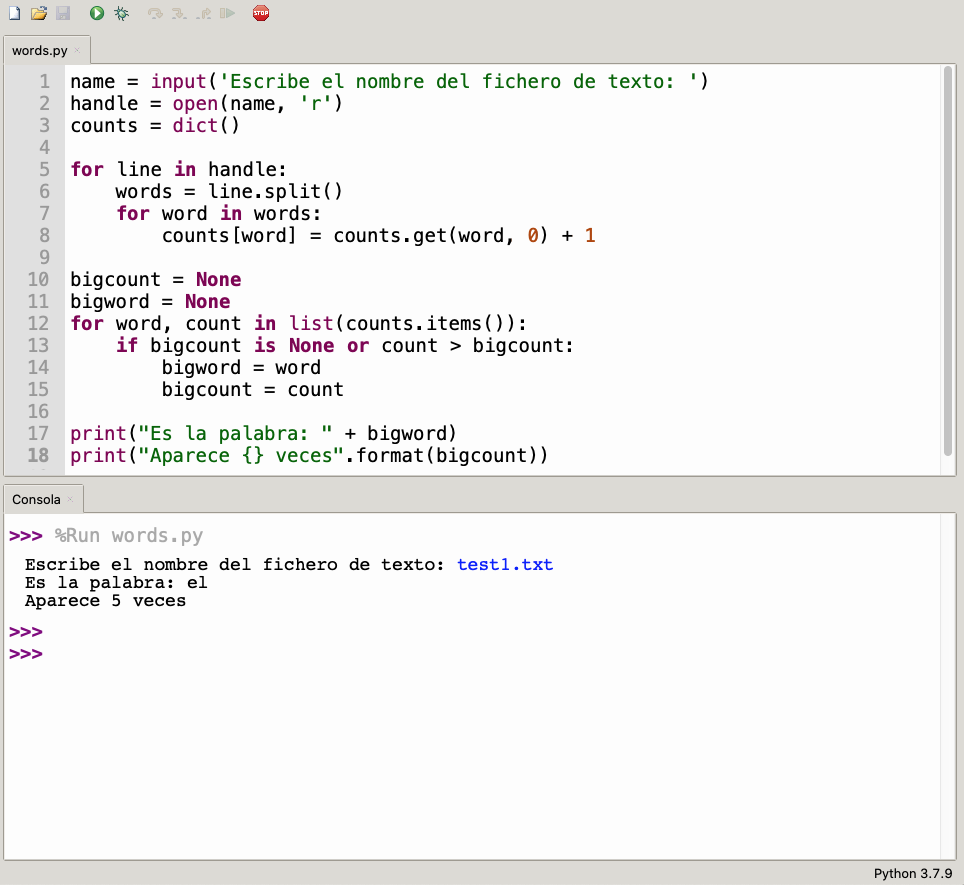
\includegraphics[width=0.85\textwidth]{images/Thonny-execute-words.png}
    \caption{Haciendo tests del programa}
    \label{fig:Thonny-execute-words}
\end{figure}



\index{programa}
Este es un buen ejemplo de cómo Python y el lenguaje Python actúan como
un intermediario entre tú (el usuario) y el programador.
Python es un medio para que intercambiemos secuencias de instrucciones útiles (es decir, programas) en un lenguaje común que puede ser usado por cualquiera que instale Python en su ordenador. Así que ninguno de nosotros está hablando \emph{con Python}, sino que estamos comunicándonos uno con el otro \emph{a través de} Python.






\hypertarget{los-bloques-de-construccion-de-los-programas}{%
\section{Los bloques de construcción de los
programas}\label{los-bloques-de-construccion-de-los-programas}}

En los próximos capítulos, aprenderemos más sobre el vocabulario, la
estructura de las frases y de los párrafos y la estructura de los
relatos en Python. Aprenderemos cuáles son las poderosas capacidades de
Python y cómo combinar esas capacidades entre sí para crear programas
útiles.

Hay ciertos patrones conceptuales de bajo nivel que se usan para
estructurar los programas. Esas estructuras no son exclusivas de Python,
sino que forman parte de cualquier lenguaje de programación, desde el
código máquina hasta los lenguajes de alto nivel.

\begin{description}
\tightlist
\item[entrada]
Obtener datos del ``mundo exterior''. Puede consistir en leer datos
desde un fichero, o incluso desde algún tipo de sensor, como un
micrófono o un GPS. En nuestros primeros programas, las entradas van a
provenir del usuario, que introducirá los datos a través del teclado.
\item[salida]
Mostrar los resultados del programa en una pantalla, almacenarlos en un
fichero o incluso es posible enviarlos a un dispositivo como un altavoz
para reproducir música o leer un texto.
\item[ejecución secuencial]
Ejecutar una sentencia tras otra en el mismo orden en que se van
encontrando en el \emph{script}.
\item[ejecución condicional]
Comprobar ciertas condiciones y luego ejecutar u omitir una secuencia de
sentencias.
\item[ejecución repetida]
Ejecutar un conjunto de sentencias varias veces, normalmente con algún
tipo de variación.
\item[reutilización]
Escribir un conjunto de instrucciones una vez, darles un nombre y así
poder reutilizarlas luego cuando se necesiten en cualquier punto de tu
programa.
\end{description}

Parece demasiado simple para ser cierto, y por supuesto nunca es tan
sencillo. Es como si dijéramos que andar es simplemente ``poner un pie
delante del otro''. El ``arte'' de escribir un programa es componer y
entrelazar juntos esos elementos básicos muchas veces hasta conseguir al
final algo que resulte útil para sus usuarios.

El programa para contar palabras que vimos antes utiliza al mismo tiempo
todos esos patrones excepto uno.

\hypertarget{quuxe9-cosas-pueden-ir-mal}{%
\section{¿Qué cosas pueden ir
mal?}\label{quuxe9-cosas-pueden-ir-mal}}

Como vimos en nuestra anterior conversación con Python, debemos
comunicarnos con mucha precisión cuando escribimos código Python. El
menor error provocará que Python se niegue a hacer funcionar tu
programa.

Los programadores novatos a menudo se toman el hecho de que Python no
permita cometer errores como la prueba definitiva de que es perverso,
odioso y cruel. A pesar de que a Python parece gustarle todos los demás,
es capaz de identificar a los novatos en concreto, y les guarda un gran
rencor. Debido a ello, toma sus programas perfectamente escritos, y los
rechaza, considerándolos como ``inservibles'', sólo para atormentarlos.

\begin{Verbatim}[frame=single]
>>> primt'¡Hola, mundo!'
  File "<pyshell>", line 1
    primt'¡Hola, mundo!'
                       ^
SyntaxError: invalid syntax
>>> primt ('Hola, mundo')
Traceback (most recent call last):
  File "<pyshell>", line 1, in <module>
NameError: name 'primt' is not defined
>>> ¡Te odio, Python!
  File "<pyshell>", line 1
    ¡Te odio, Python!
      ^
SyntaxError: invalid character in identifier
>>> si sales fuera, te daré una lección
  File "<pyshell>", line 1
    si sales fuera, te daré una lección
           ^
SyntaxError: invalid syntax
>>> 
\end{Verbatim}

No es mucho lo que se gana discutiendo con Python. Solo es una
herramienta. No tiene emociones, es feliz y está preparado para servirte
en el momento que lo necesites. Sus mensajes de error parecen crueles,
pero simplemente se trata de una petición de ayuda del propio Python. Ha
examinado lo que has tecleado, y sencillamente no es capaz de entender
lo que has escrito.

Python se parece mucho a un perro, te quiere incondicionalmente,
entiende algunas pocas palabras clave, te mira con una mirada dulce en
su cara(\texttt{\textgreater{}\textgreater{}\textgreater{}}), y espera
que le digas algo que él pueda comprender. Cuando Python dice
``SyntaxError: invalid syntax'' (Error de sintaxis: sintaxis inválida),
tan solo está agitando su cola y diciendo: ``Creo que has dicho algo,
pero no te entiendo; de todos modos, por favor, sigue hablando conmigo
(\texttt{\textgreater{}\textgreater{}\textgreater{}}).''

A medida que tus programas vayan aumentando su complejidad, te
encontrarás con tres tipos de errores generales:

\begin{description}
\tightlist
\item[Errores de sintaxis (Syntax errors)]
Estos son los primeros errores que cometerás y también los más fáciles
de solucionar. Un error de sintaxis significa que has violado las reglas
``gramaticales'' de Python. Python hace todo lo que puede para señalar
el punto exacto, la línea y el carácter donde ha detectado el fallo. Lo
único complicado de los errores de sintaxis es que a veces el error que
debe corregirse está en realidad en una línea anterior a la cual Python
\emph{detectó} ese fallo. De modo que la línea y el carácter que Python
indica en un error de sintaxis pueden ser tan sólo un punto de partida
para tu investigación.
\item[Errores lógicos]
Se produce un error lógico cuando un programa tiene una sintaxis
correcta, pero existe un error en el orden de las sentencias o en la
forma en que están relacionadas unas con otras. Un buen ejemplo de un
error lógico sería: ``toma un trago de tu botella de agua, ponla en tu
mochila, camina hasta la biblioteca y luego vuelve a enroscar la tapa en
la botella.''
\item[Errores semánticos]
Un error semántico ocurre cuando la descripción que has brindado de los
pasos a seguir es sintácticamente perfecta y está en el orden correcto,
pero sencillamente hay un error en el programa. El programa es correcto,
pero no hace lo que tú \emph{pretendías} que hiciera. Un ejemplo podría
ser cuando le das indicaciones a alguien sobre cómo llegar a un
restaurante, y le dices ``\ldots cuando llegues a la intersección con la
gasolinera, gira a la izquierda, continúa durante otro kilómetro y el
restaurante es el edificio rojo que encontrarás a tu izquierda.''. Tu
amigo se retrasa y te llama para decirte que está en una granja dando
vueltas alrededor de un granero, sin rastro alguno de un restaurante.
Entonces le preguntas ``¿giraste a la izquierda o la derecha?'', y te
responde ``Seguí tus indicaciones al pie de la letra, dijiste que girara
a la izquierda y continuar un kilómetro desde la gasolinera.'', entonces
le respondes ``Lo siento mucho, porque a pesar de que mis indicaciones
fueron sintácticamente correctas, tristemente contenían un pequeño pero
indetectado error semántico.''.
\end{description}

Insisto en que, ante cualquiera de estos tres tipos de errores, Python
únicamente hace lo que está a su alcance por seguir al pie de la letra
lo que tú le has pedido que haga.

Errores de sintaxis los encuentra el interprete de Python porque
verifica las reglas grammaticales del lenguaje.

Errores lógicos y semanticos solo los podemos encontrar ejecutando y
probando (testeando) nuestro programa. Como hemos indicando ya antes,
siempre cuando estas programando tienes que testear para asegurar que tu
código hace lo que esperas.

\hypertarget{depurando-los-programas}{%
\section{Testing y depuración de los programas}\label{depurando-los-programas}}

Cuando hacemos testing de un programa ejecutamos el programa para ver lo que sale y comparar esta salida con lo que esperamos que tiene que salir.
%
Cuando Python muestra un error, o devuelve un resultado
diferente al que esperabas, empieza una búsqueda de la causa del error. Depurar es el proceso de encontrar la causa o el origen de ese error en tu código. Cuando depuras un programa, y especialmente cuando tratas con un \emph{bug} algo difícil de solucionar, existen cuatro cosas por hacer:

\begin{description}
\tightlist
\item[leer]
Revisar tu código, leerlo de nuevo, y asegurarte de que ahí está
expresado de forma correcta lo que quieres decir.
\item[ejecutar]
Prueba haciendo cambios y ejecutando diferentes versiones. Con
frecuencia, si muestras en tu programa lo correcto en el lugar indicado,
el problema se vuelve obvio, pero en ocasiones debes invertir algo de
tiempo hasta conseguirlo.
\item[pensar detenidamente]
¡Toma tu tiempo para pensar!, ¿A qué tipo de error corresponde:
sintaxis, en tiempo de ejecución, semántico?, ¿Qué información puedes
obtener de los mensajes de error, o de la salida del programa?, ¿Qué
tipo de errores podría generar el problema que estás abordando?, ¿Cuál
fue el último cambio que hiciste, antes de que se presentara el
problema?
\item[retroceder]
En algún momento, lo mejor que podrás hacer es dar marcha atrás,
deshacer los cambios recientes hasta obtener de nuevo un programa que
funcione y puedas entender. Llegado a ese punto, podrás continuar con tu
trabajo.
\end{description}

Algunas veces, los programadores novatos se quedan estancados en una de
estas actividades y olvidan las otras. Encontrar un \emph{bug} requiere
leer, ejecutar, pensar detenidamente y algunas veces retroceder. Si te
bloqueas en alguna de estas actividades, prueba las otras. Cada
actividad tiene su procedimiento de análisis.

\index{error tipográfico}

Por ejemplo, leer tu código podría ayudar si el problema es un error
tipográfico, pero no si es uno conceptual. Si no comprendes lo que hace
tu programa, puedes leerlo 100 veces y no encontrarás el error, puesto
que dicho error está en tu mente.

\index{depuración experimental}

Experimentar puede ayudar, especialmente si ejecutas pequeñas pruebas.
Pero si experimentas sin pensar o leer tu código, podrías caer en un
patrón que llamo ``programación de paseo aleatorio'', que es el proceso
de realizar cambios al azar hasta que el programa logre hacer lo que
debería. No hace falta mencionar que este tipo de programación puede
tomar mucho tiempo.

\index{programación de paseo aleatorio}
\index{plan de desarrollo!programación de paseo aleatorio}

Debes tomar el tiempo suficiente para pensar. Depurar es como una
ciencia experimental. Debes plantear al menos una hipótesis sobre qué
podría ser el problema. Si hay dos o más posibilidades, piensa en alguna
prueba que pueda ayudarte a descartar una de ellas.

Descansar y conversar ayuda a estimular el pensamiento. Si le explicas
el problema a alguien más (o incluso a tí mismo), a veces encontrarás la
respuesta antes de terminar la pregunta.

Pero incluso las mejores técnicas de depuración fallarán si hay
demasiados errores, o si el código que intentas mejorar es demasiado
extenso y complicado. Algunas veces la mejor opción es retroceder, y
simplificar el programa hasta que obtengas algo que funcione y puedas
entender.

Por lo general, los programadores novatos son reacios a retroceder
porque no soportan tener que borrar una línea de código (incluso si está
mal). Si te hace sentir mejor, prueba a copiar tu programa en otro
archivo antes de empezar a modificarlo. De esa manera, puedes recuperar
poco a poco pequeñas piezas de código que necesites.

\index{Kill your darlings}\index{matar a tus favoritos}
''Kill your darlings'', o ''matar a tus favoritos'' en español, es un concepto fundamental en el proceso de aprendizaje de programación y en el desarrollo del pensamiento computacional. Esta expresión se refiere a la idea de que, en el camino de mejorar tus habilidades y crear soluciones más eficientes, a veces es necesario eliminar partes de tu código que pueden parecer valiosas o significativas, pero que en realidad no contribuyen al objetivo final o pueden estar introduciendo complejidad innecesaria.

Cuando estás aprendiendo a programar, es fácil sentir apego por las piezas de código que has creado, especialmente si has invertido tiempo y esfuerzo en ellas. Sin embargo, eliminar código redundante, ineficiente o incorrecto es una habilidad crucial. No solo mejora la legibilidad y mantenibilidad de tu código, sino que también refleja tu crecimiento como programador.

Entender que eliminar código no es una pérdida, sino una oportunidad para mejorar, es un paso importante en la evolución como programador. Cada vez que decides eliminar un fragmento de código, estás demostrando que estás dispuesto a aprender de tus errores y a optimizar tus soluciones. Esta mentalidad te permitirá crear programas más sólidos, eficientes y comprensibles, lo cual es esencial en el mundo de la programación.

En resumen, ''kill your darlings'' resalta la importancia de la humildad y la adaptabilidad en el proceso de aprendizaje de programación. No se trata solo de escribir código, sino de aprender a refactorizar, mejorar y optimizar constantemente, incluso si eso implica eliminar el trabajo en el que has invertido tiempo. Cada línea de código que eliminas ha contribuido a tu camino de aprendizaje.




\hypertarget{el-camino-del-aprendizaje}{%
\section{El camino del aprendizaje}\label{el-camino-del-aprendizaje}}

Según vayas avanzando con el curso, no te asustes si los conceptos no
parecen encajar bien unos con otros al principio. Cuando estabas
aprendiendo a hablar, no supuso un problema que durante los primeros
años solo pudieras emitir lindos balbuceos. Y también fue normal que te
llevara seis meses pasar de un vocabulario simple a frases simples, y
que te llevara 5-6 años más pasar de frases a párrafos, y que todavía
tuvieran que transcurrir unos cuantos años más hasta que fuiste capaz de
escribir tu propia historia corta interesante.

Pretendemos que aprendas Python rápidamente, por lo que te enseñaremos
todo al mismo tiempo durante los próximos capítulos. Aún así, ten en
cuenta que el proceso es similar a aprender un idioma nuevo, que lleva
un tiempo absorber y comprender antes de que te resulte familiar. Eso
produce cierta confusión, puesto que revisaremos en distintas ocasiones
determinados temas, y trataremos que de esa manera puedas visualizar los
pequeños fragmentos que componen esta obra completa. A pesar de que el
libro está escrito de forma lineal, no dudes en ser no lineal en la
forma en que abordes las materias. Avanza y retrocede, y lee a veces por
encima. Al ojear material más avanzado sin comprender del todo los
detalles, tendrás una mejor comprensión del ``¿por qué?'' de la
programación. Al revisar el material anterior e incluso al realizar
nuevamente los ejercicios previos, te darás cuenta que ya has aprendido
un montón de cosas, incluso si el tema que estás examinando en ese
momento parece un poco difícil de abordar.

Normalmente, cuando uno aprende su primer lenguaje de programación, hay
unos pocos momentos ``¡A-já!'' estupendos, en los cuales puedes levantar
la vista de la roca que estás machacando con martillo y cincel,
separarte unos pasos y comprobar que lo que estás intentando construir
es una maravillosa escultura.

Si algo parece particularmente difícil, generalmente no vale la pena
quedarse mirándolo toda la noche. Respira, toma una siesta, come algo,
explícale a alguien (quizás a tu perro) con qué estás teniendo
problemas, y después vuelve a observarlo con un perspectiva diferente.
Te aseguro que una vez que aprendas los conceptos de la programación en
el libro, volverás atrás y verás que en realidad todo era fácil,
elegante y que simplemente te ha llevado un poco de tiempo llegar a
absorberlo.


Si llegas a un punto en el que te sientes bloqueado y no estás seguro de cómo avanzar, recuerda que siempre puedes solicitar una cita para una tutoría con tu profesora. Ya sea en persona o en línea, también puedes enviarle un mensaje a través de WhatsApp, Telegram o TEAMs. No esperes demasiado tiempo para hacerlo; esperar hasta, por ejemplo, dos días antes de un examen, no es el momento más adecuado. Aprovechar la oportunidad de aclarar tus dudas y recibir orientación puede marcar una gran diferencia en tu comprensión y éxito en el aprendizaje.

\hypertarget{glosario_introduccion}{%
\section{Glosario}\label{glosario_introduccion}}

\begin{description}
\tightlist
\item[algoritmo]
Un algoritmo es una secuencia de instrucciones especificas de las
acciones que ha de ejecutar y en qué orden para completar una tarea
determinada. \index{algoritmo}
\item[bug]
Un error en un programa. \index{bug}
\item[código fuente]
Un programa en un lenguaje de alto nivel. \index{código fuente}
\item[código máquina]
El lenguaje de más bajo nivel para el software, es decir, el lenguaje
que es directamente ejecutado por la unidad central de procesamiento
(CPU). \index{código máquina}
\item[compilar]
Traducir un programa completo escrito en un lenguaje de alto nivel a un
lenguaje de bajo nivel, para dejarlo listo para una ejecución posterior.
\index{compilar}
\item[error semántico]
Un error dentro de un programa que provoca que haga algo diferente de lo
que pretendía el programador. \index{error semántico}
\item[función print]
Una instrucción que hace que el intérprete de Python muestre un valor en
la pantalla. \index{print (función)} \index{función!print}
\item[indicador de línea de comandos (\emph{prompt})]
Cuando un programa muestra un mensaje y se detiene para que el usuario
teclee algún tipo de dato. \index{prompt}
\index{indicador de línea de comandos}
\item[interpretar]
Ejecutar un programa escrito en un lenguaje de alto nivel traduciéndolo
línea a línea. \index{interpretar}
\item[lenguaje de alto nivel]
Un lenguaje de programación como Python, que ha sido diseñado para que
sea fácil de leer y escribir por las personas.
\index{lenguaje de alto nivel}
\item[lenguaje de bajo nivel]
Un lenguaje de programación que está diseñado para ser fácil de ejecutar
para un ordenador; también recibe el nombre de ``código máquina'',
``lenguaje máquina'' o ``lenguaje ensamblador''.
\index{lenguaje de bajo nivel}
\item[memoria principal]
Almacena los programas y datos. La memoria principal pierde su
información cuando se desconecta la alimentación.
\index{memoria principal}
\item[memoria secundaria]
Almacena los programas y datos y mantiene su información incluso cuando
se interrumpe la alimentación. Es generalmente más lenta que la memoria
principal. Algunos ejemplos de memoria secundaria son las unidades de
disco y memorias flash que se encuentran dentro de los dispositivos USB.
\index{memoria secundaria}
\item[modo interactivo]
Un modo de usar el intérprete de Python, escribiendo comandos y
expresiones directamente en el indicador de la línea de comandos.
\index{modo interactivo}
\item[parsear]
Examinar un programa y analizar la estructura sintáctica.
\index{parsear}
\item[portabilidad]
Es la propiedad que poseen los programas que pueden funcionar en más de
un tipo de ordenador. \index{portabilidad}
\item[programa]
Un conjunto de instrucciones que indican cómo realizar algún tipo de
cálculo. \index{programa}
\item[resolución de un problema]
El proceso de formular un problema, encontrar una solución, y mostrar
esa solución. \index{resolución de un problema}
\item[semántica]
El significado de un programa. \index{semántica}
\item[testing, testear (probar)]
Ejecutar tu programa para asegurar que haga lo que esperas que haga.
\index{testing}\index{testear}\index{probar}
\item[unidad central de procesamiento]
El corazón de cualquier ordenador. Es lo que ejecuta el software que
escribimos. También recibe el nombre de ``CPU'' por sus siglas en inglés
(\emph{Central Processsing Unit}), o simplemente, ``el procesador''.
\index{unidad central de procesamiento} \index{CPU}
\end{description}


